\documentclass[11pt,fontset=none,scheme=plain]{ctexart}

\setCJKmainfont{NotoSerifSC-Regular.ttf}[
  Path = ./,
  Script = CJK,
  BoldFont = NotoSerifSC-SemiBold.ttf,
  ItalicFont = NotoSerifSC-Regular.ttf,
  BoldItalicFont = NotoSerifSC-SemiBold.ttf
]
\setCJKsansfont{NotoSerifSC-Regular.ttf}[
  Path = ./,
  Script = CJK,
  BoldFont = NotoSerifSC-SemiBold.ttf
]
\setCJKmonofont{NotoSerifSC-Regular.ttf}[
  Path = ./,
  Script = CJK,
  BoldFont = NotoSerifSC-SemiBold.ttf
]

\usepackage[margin=1in]{geometry}
\usepackage{amsmath}
\usepackage{booktabs}
\usepackage{graphicx}
\usepackage{caption}
\usepackage{placeins}

\makeatletter
\setlength{\@fptop}{8pt}
\setlength{\@fpbot}{0pt plus 1fil}
\makeatother

\captionsetup{font=small,skip=8pt}
\AtBeginDocument{%
  \renewcommand{\tablename}{表}%
  \renewcommand{\figurename}{图}%
}
\setlength{\parskip}{0.45em}
\setlength{\parindent}{0pt}

\title{第一阶段：静态 OLS 对冲残差上的 OU 估计\\[0.3em]
\large 511090 对 TL 期货}
\date{2026 年 9 月 29 日}

\begin{document}
\maketitle

本文是 511090 与 TL 这一配对的第一阶段。组合交易的是对冲之后的残差，并把残差建模为奥恩斯坦--乌伦贝克过程。在静态残差上，样本外比较两种 OU 参数估计：每 180 分钟更新一次的滚动 OLS 窗口，以及卡尔曼滤波。后者的过程噪声、开仓带和平仓带都在训练窗口上选定。

\section{OU 配对交易}
\label{sec:ou}

ETF 511090 与 TL 期货走势相近，组合交易的是用一方对冲另一方之后留下的残差。前提是残差会回到均衡水平。残差高于均衡时，组合卖出残差；低于均衡时，组合买入残差；一旦回到带内，组合即平仓。

残差 $X$ 服从奥恩斯坦--乌伦贝克过程
\begin{equation}
dX_t = \theta(\mu - X_t)\,dt + \sigma\,dW_t.
\end{equation}
$\theta > 0$ 是回归速度，$\mu$ 是均衡水平，$\sigma$ 是扩散系数。均衡偏离为
\begin{equation}
\sigma_{\mathrm{eq}} = \frac{\sigma}{\sqrt{2\theta}},
\end{equation}
信号则是用这个尺度衡量的、离开均衡的距离，
\begin{equation}
z = \frac{X - \mu}{\sigma_{\mathrm{eq}}}.
\end{equation}
半衰期为 $\ln 2 / \theta$。

OU 过程的 AR(1) 形式为
\begin{equation}
X_{t+1} = a X_t + b + \varepsilon_t,
\end{equation}
其中 $a = e^{-\theta}$，$b = \mu(1-a)$。$\Delta t$ 取一分钟时，换算回过程参数为
\begin{align}
\theta &= -\ln a, &
\mu &= \frac{b}{1-a}, &
\sigma &= \sigma_\varepsilon \sqrt{\frac{2\theta}{1-a^2}}.
\end{align}

\section{组合}

信号是第~\ref{sec:ou}~节的 $z$。$z$ 高于开仓带时做空价差：卖出 ETF、买入 TL。$z$ 低于开仓带的相反数时做多价差，方向相反。$|z|$ 回到平仓带以内就平仓。同一时间只持有一笔价差。仓位可以隔夜，也可以跨过午休。

开仓手数取 $\mathrm{round}(|z|)$ 手 TL，至少 1 手、至多 8 手；若 ETF 与 TL 的名义本金之和超过 1000 万，再把手数下调到限额以内。组合回到空仓之前，手数不变。一手 TL 每点价值 1 万元，与 1 万股 ETF 每点的金额相同，所以用来跟踪 $X$ 的股数是 $\mathrm{round}(\mathrm{lots}\times 10{,}000/\beta)$。（$\beta$ 见后文。）

ETF 手续费为名义本金的 0.5 bp，TL 手续费为名义本金的 0.25 bp（按每手 3 元估算），开仓收一次，平仓再收一次。

起始资金为 1000 万，与名义本金上限相同。绝对收益是这笔资金的总变动。年化收益按 $252/63$ 复利。夏普比率是日收益均值除以样本标准差，再乘以 $\sqrt{252}$，不含无风险利率。最大回撤是资金从前期高点到其后低点的最大跌幅。一笔交易指一次完成的往返。

\section{对冲}

上面的过程描述的是 $X$，而 $X$ 要先做完对冲才存在。ETF 与 TL 期货可以有共同的漂移；被假定会回归的序列，是 ETF 最新价中 TL 最新价解释不了的那一部分，
\begin{equation}
X = P_{\mathrm{ETF}} - \alpha - \beta P_{\mathrm{TL}}.
\end{equation}
$\beta$ 是对冲 ETF 一个点所对应的 TL 点数。AR(1) 拟合的是这个残差，所以 $\alpha$ 和 $\beta$ 要先定下来。在此之前，$z$ 没有定义。后文的 OU 估计，用的都是对冲已经给出的残差；下面用同一个 OU 估计来比较这两种对冲。

样本是 ETF 511090 与 TL 期货主力连续合约（换月拼接已经完成），覆盖 2025 年 7 月 1 日至 12 月 30 日双方共同交易的 125 个交易日。两路行情都只保留共同交易时段，即 09:30--11:30 与 13:00--15:00。TL 报价更密，用向后 as-of 对齐到 ETF 的时间戳上，因此每一行都落在 ETF 的三秒网格上。训练窗口是前 62 个交易日，7 月 1 日至 9 月 24 日。测试期是其余 63 个交易日，9 月 25 日至 12 月 30 日。

\subsection{静态对冲与滚动对冲}

两种对冲都在降采样到 1 分钟的最新价上拟合。静态 OLS 只在训练窗口上估计，系数用于每一行三秒行情：
\[
\hat\beta = 1.0557, \qquad \hat\alpha = -2.5923.
\]
滚动 OLS 每个交易日用此前 20 个交易日的 1 分钟最新价重估 $\alpha$ 和 $\beta$。前三个月里，这个 beta 介于 0.795 与 1.143 之间。

训练窗口上，滚动残差比静态残差回归得更快，半衰期为 200 分钟，静态残差为 304 分钟。静态的这组数字来自对该残差做的一次 AR(1) OLS，共 14{,}756 对：$a = 0.99772$，$\mu = -0.027$，$\sigma = 0.0147$，$\sigma_{\mathrm{eq}} = 0.218$。

随后用第~\ref{sec:trailing}~节同一个滚动 OLS 的 OU 估计，分别在两种对冲上交易。滚动对称组合的收益为 0.371\%，夏普比率为 3.57；静态对称组合的收益为 0.997\%，夏普比率为 6.44。看来滚动对冲对近期窗口适应过度，把可交易的优势吃掉了。表~\ref{tab:hedge} 以静态拟合为基准，后文的对冲都固定在这一组系数上。

\begin{table}[ht]
\centering
\caption{样本外组合。对冲分别为静态与滚动，OU 估计为过去五个交易日的滚动 OLS。}
\label{tab:hedge}
\begin{tabular}{llrrrrr}
\toprule
对冲 & 方向 & 收益 & 年化 & 夏普 & 最大回撤 & 笔数 \\
\midrule
静态 & 空头 & 0.685\% & 2.769\% & 4.62 & $-0.086\%$ & 21 \\
静态 & 多头 & 0.226\% & 0.907\% & 3.35 & $-0.268\%$ & 16 \\
静态 & 对称 & 0.997\% & 4.047\% & 6.44 & $-0.086\%$ & 36 \\
滚动 & 空头 & 0.070\% & 0.279\% & 1.42 & $-0.126\%$ & 10 \\
滚动 & 多头 & 0.301\% & 1.212\% & 3.17 & $-0.138\%$ & 12 \\
滚动 & 对称 & 0.371\% & 1.493\% & 3.57 & $-0.138\%$ & 22 \\
\bottomrule
\end{tabular}
\end{table}

\FloatBarrier
\section{滚动 OLS}
\label{sec:trailing}

测试期内，每累计满 180 根一分钟 K 线，就重新估计一次 $\mu$、$\sigma$ 和 $\theta$。窗口是最近五个交易日，共 1{,}200 根一分钟 K 线；回归用第~\ref{sec:ou}~节的 AR(1)，隔夜和午休都不计入 $\Delta t$。新参数从窗口最后一根 K 线的下一分钟起使用。若某个窗口的 AR(1) 系数不在 $(0,1)$ 内，则保留上一次的拟合。静态价差的 85 个窗口里，有 3 个是这样。开仓带固定为 2，平仓带固定为 0.5。

\section{卡尔曼滤波}

滤波估计的是静态价差的 AR(1) 系数，对冲保持静态拟合。状态 $(a_t, b_t)$ 按随机游走建模，观测则是价差的下一分钟价格，
\begin{equation}
\begin{pmatrix} a_t \\ b_t \end{pmatrix}
=
\begin{pmatrix} a_{t-1} \\ b_{t-1} \end{pmatrix}
+ w_t,
\qquad
S_t = a_t S_{t-1} + b_t + v_t.
\end{equation}
过程噪声 $w_t$ 的协方差为对角阵 $\mathrm{diag}(q_a, q_b)$，观测噪声 $v_t$ 的方差为 $R$。

$R$ 取训练窗口 AR(1) 的残差方差，从训练到测试全程固定。在 14{,}756 个训练样本上，残差标准差为 $\sigma_\varepsilon = 0.01469$，因此
\[
R = \sigma_\varepsilon^2 = 2.158\times 10^{-4}.
\]
$P_0$ 是第一分钟状态的协方差，即这两个系数的 OLS 抽样协方差 $\sigma_\varepsilon^2 (X^{\top} X)^{-1}$。$X$ 的两列分别是滞后价差和常数项：
\[
P_0 =
\begin{pmatrix}
3.678\times 10^{-7} & -2.100\times 10^{-11} \\
-2.100\times 10^{-11} & 1.463\times 10^{-8}
\end{pmatrix}.
\]
状态初值就是这次拟合，$a = 0.99772$，$b = -6.132\times 10^{-5}$。每次更新后，将 $\hat a$ 截断到 $[0.001, 0.999]$。某一分钟上保存的状态，取的是该分钟价格进入滤波之前的值。午休或隔夜只把上一时刻的后验带过去，不叠加过程噪声。$R$ 和 $P_0$ 保持训练期的取值，滤波状态则连续递推，覆盖整个测试期。

搜索调整的是过程噪声和带宽规则。$R$、$P_0$、初始状态和对冲都保持训练拟合。带宽随滤波结果变化，
\begin{equation}
z_t = z_0
\left(\frac{\tau_{1/2,t}}{\bar\tau_{1/2}}\right)^{\gamma_\tau}
\left(\frac{\sigma_t}{\bar\sigma}\right)^{\gamma_\sigma},
\end{equation}
开仓和平仓各有一组 $(z_0, \gamma_\tau, \gamma_\sigma)$。$\tau_{1/2} = \ln 2 / \theta$，$\sigma$ 为扩散系数，二者都取自该次试验的滤波路径。锚点 $\bar\tau_{1/2}$ 与 $\bar\sigma$ 是样本内逐分钟路径的中位数，样本外沿用训练期的这两个中位数。在锚点处两个因子都等于 1，带宽就等于 $z_0$。弹性取 0 时，对应因子在整条路径上保持为 1。弹性为正时，半衰期或 $\sigma$ 高于其锚点则带宽提高，低于锚点则带宽降低。

八个量各自从表~\ref{tab:search} 的闭区间中抽取。两个对数区间限制 $a$ 和 $b$ 游走的快慢。弹性不超过 0.6，因此半衰期或 $\sigma$ 翻倍时，带宽至多乘以 $2^{0.6} \approx 1.52$。

\begin{table}[ht]
\centering
\caption{盒约束。每个待搜索的量都从这个区间中抽取。}
\label{tab:search}
\begin{tabular}{llc}
\toprule
参数 & 含义 & 区间 \\
\midrule
$\log_{10} q_a$ & $a$ 的过程方差 & $[-10,\,-5]$ \\
$\log_{10} q_b$ & $b$ 的过程方差 & $[-8,\,-3]$ \\
$z_0$ 开仓 & 锚点处的开仓带 & $[1.2,\,2.5]$ \\
$z_0$ 平仓 & 锚点处的平仓带 & $[0.1,\,0.6]$ \\
$\gamma_\tau$ 开仓 & 开仓带对半衰期的弹性 & $[0,\,0.6]$ \\
$\gamma_\tau$ 平仓 & 平仓带对半衰期的弹性 & $[0,\,0.6]$ \\
$\gamma_\sigma$ 开仓 & 开仓带对 $\sigma$ 的弹性 & $[0,\,0.6]$ \\
$\gamma_\sigma$ 平仓 & 平仓带对 $\sigma$ 的弹性 & $[0,\,0.6]$ \\
\bottomrule
\end{tabular}
\end{table}

公式算出带宽之后，每一分钟再施加表~\ref{tab:bounds} 的三条约束。公式给出的开仓带小于 1 时抬到 1，平仓带小于 0.05 时抬到 0.05，再把平仓带限制到至少比开仓带低 0.8。这三条对每次试验都相同。因此在锚点处，开仓 $z_0 = 1.2$、平仓 $z_0 = 0.6$ 的试验，实际交易的平仓带是 0.4。

\begin{table}[ht]
\centering
\caption{公式之后、每一分钟都施加在两条带宽上的约束。}
\label{tab:bounds}
\begin{tabular}{ll}
\toprule
约束 & 规则 \\
\midrule
开仓下限 & $z^{\mathrm{entry}} \ge 1$ \\
平仓下限 & $z^{\mathrm{exit}} \ge 0.05$ \\
间距 & $z^{\mathrm{entry}} - z^{\mathrm{exit}} \ge 0.8$ \\
\bottomrule
\end{tabular}
\end{table}

训练交易日按时间分成三段，长度分别为 21、21 和 20 个交易日：7 月 1 日至 29 日、7 月 30 日至 8 月 27 日、8 月 28 日至 9 月 24 日。每一段的对称组合都从空仓开始。记 $S_1$、$S_2$ 和 $S_3$ 为这三段的夏普比率。搜索最大化
\begin{equation}
J = \bar S - s,
\qquad
\bar S = \frac{S_1 + S_2 + S_3}{3},
\qquad
s = \sqrt{\frac{(S_1 - \bar S)^2 + (S_2 - \bar S)^2 + (S_3 - \bar S)^2}{3}}.
\end{equation}
三段的夏普都高、而且三个数彼此接近时，$J$ 才高。Optuna 的 TPE 搜索共 300 次试验，前 40 次随机抽取，选中的是表~\ref{tab:chosen} 中的试验。

\begin{table}[ht]
\centering
\caption{训练窗口上选中的试验，及其目标函数取值。}
\label{tab:chosen}
\begin{tabular}{lr}
\toprule
量 & 取值 \\
\midrule
$\log_{10} q_a$ & $-5.10$ \\
$q_a$ & $7.95\times 10^{-6}$ \\
$\log_{10} q_b$ & $-5.65$ \\
$q_b$ & $2.23\times 10^{-6}$ \\
$z_0$ 开仓 & 2.421 \\
$z_0$ 平仓 & 0.508 \\
$\gamma_\tau$ 开仓 & 0.507 \\
$\gamma_\tau$ 平仓 & 0.085 \\
$\gamma_\sigma$ 开仓 & 0.425 \\
$\gamma_\sigma$ 平仓 & 0.187 \\
\midrule
夏普，7 月 1 日至 29 日 & 13.13 \\
夏普，7 月 30 日至 8 月 27 日 & 13.08 \\
夏普，8 月 28 日至 9 月 24 日 & 15.85 \\
平均夏普 $\bar S$ & 14.02 \\
标准差 $s$ & 1.29 \\
目标 $J$ & 12.73 \\
\bottomrule
\end{tabular}
\end{table}

选中的 $\log_{10} q_a = -5.10$ 靠近 $[-10, -5]$ 的上沿，因此 $a$ 几乎取到了盒约束允许的最大过程方差。$\log_{10} q_b = -5.65$ 落在 $[-8, -3]$ 内部。锚点开仓 2.421 接近 $[1.2, 2.5]$ 的上沿，锚点平仓 0.508 落在 $[0.1, 0.6]$ 内部。两个锚点相差 1.91，已经宽于要求的 0.8，所以间距约束并没有改动它们。开仓弹性在半衰期上是 0.507，在 $\sigma$ 上是 0.425：回归变慢或扩散系数变大时，开仓带会放宽。平仓弹性是 0.085 和 0.187，平仓带几乎不动。

\section{样本外}

卡尔曼对称组合领先于滚动组合，收益 1.806\%、夏普比率 12.03，滚动组合则是 0.997\% 和 6.44，往返笔数 436 对 36。

\begin{table}[ht]
\centering
\caption{静态对冲上的样本外组合，2025 年 9 月 25 日至 12 月 30 日。}
\label{tab:oos}
\begin{tabular}{llrrrrr}
\toprule
估计 & 方向 & 收益 & 年化 & 夏普 & 最大回撤 & 笔数 \\
\midrule
滚动 OLS & 空头 & 0.685\% & 2.769\% & 4.62 & $-0.086\%$ & 21 \\
滚动 OLS & 多头 & 0.226\% & 0.907\% & 3.35 & $-0.268\%$ & 16 \\
滚动 OLS & 对称 & 0.997\% & 4.047\% & 6.44 & $-0.086\%$ & 36 \\
卡尔曼 & 空头 & 0.997\% & 4.046\% & 8.74 & $-0.094\%$ & 244 \\
卡尔曼 & 多头 & 0.970\% & 3.936\% & 9.84 & $-0.083\%$ & 197 \\
卡尔曼 & 对称 & 1.806\% & 7.422\% & 12.03 & $-0.093\%$ & 436 \\
\bottomrule
\end{tabular}
\end{table}

图~\ref{fig:spread} 画出静态价差和两条 $z$，图~\ref{fig:position} 画出对称组合的仓位。两张图都是一分钟最新价。价差水平在 12 月初下移。滚动的 $z$ 按 180 分钟的更新节拍跟上这次下移；卡尔曼的 $z$ 和开仓带则每分钟都在动。仓位图对应的就是这个差别：滚动组合的持仓长达数小时或数日，卡尔曼组合在当日交易时段内进出。正的手数表示空头价差。

\begin{figure}[ht]
\centering
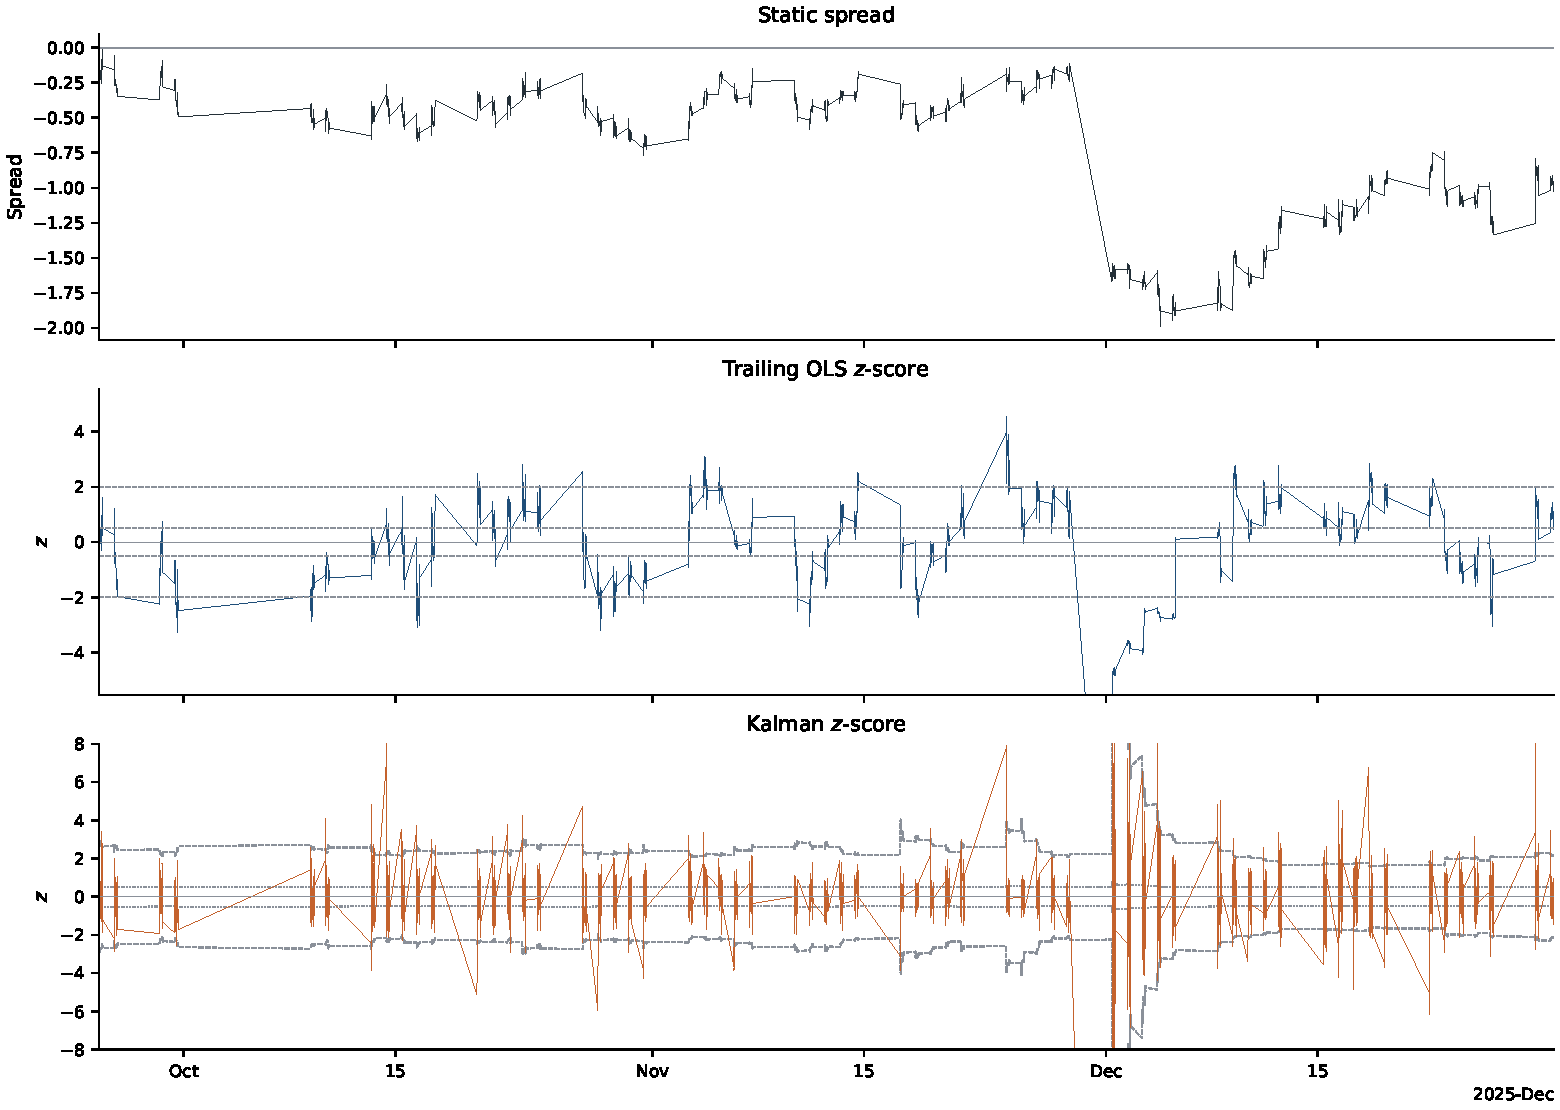
\includegraphics[width=\textwidth]{figures/spread_z.pdf}
\caption{样本外的静态价差与 $z$。滚动面板中，虚线是固定在 $\pm 2$ 和 $\pm 0.5$ 的带宽。卡尔曼面板中，虚线是动态开仓带，点线是平仓带。纵轴略去了 12 月 1 日的开盘，当时滚动 $z$ 为 $-17.9$，卡尔曼 $z$ 为 $-71.2$。卡尔曼开仓带在这次开盘达到 38.5，超出画面，在图框处被截断。}
\label{fig:spread}
\end{figure}

\begin{figure}[ht]
\centering
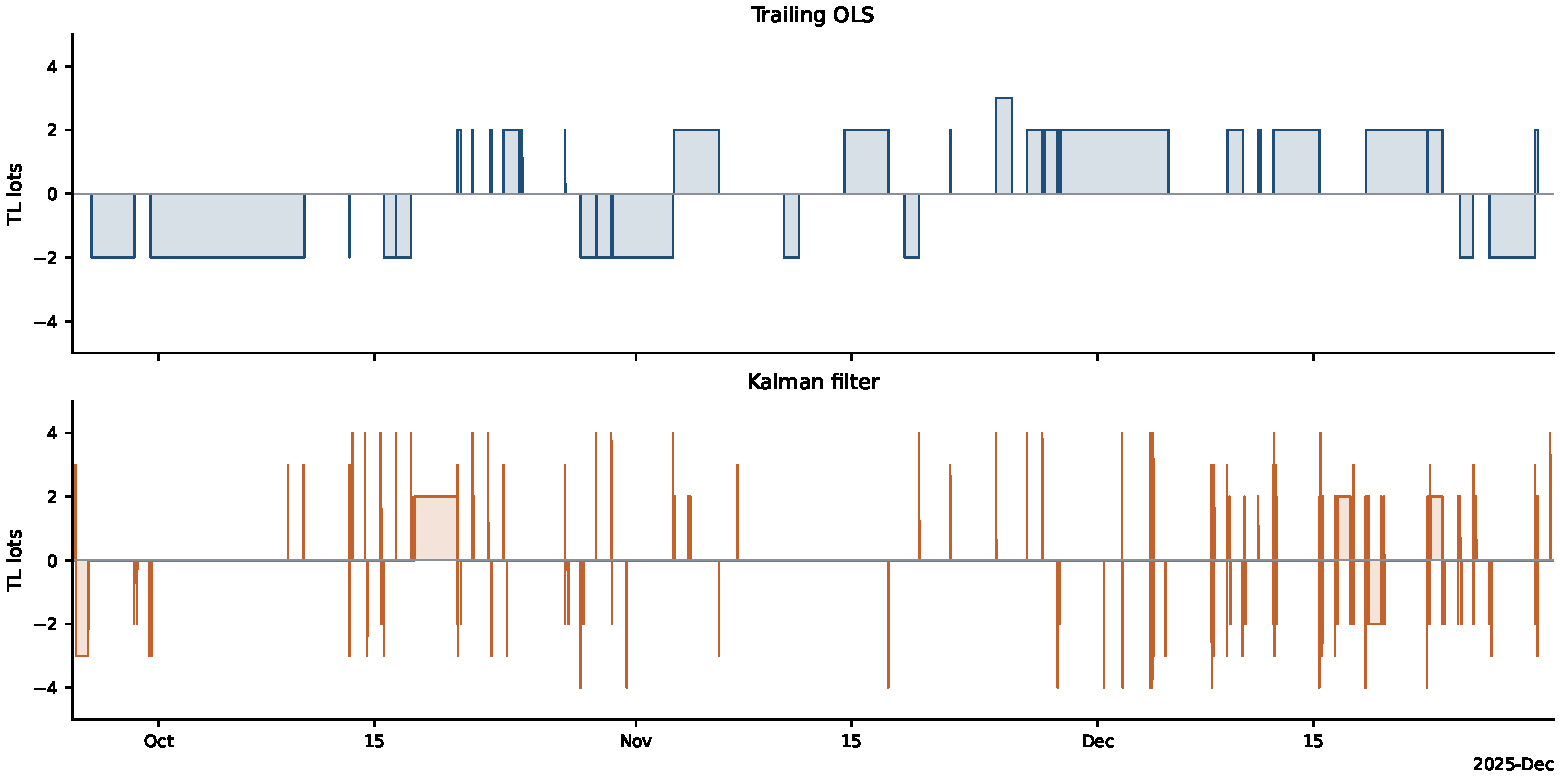
\includegraphics[width=\textwidth]{figures/position.pdf}
\caption{对称组合的带符号 TL 手数。正手数为空头价差。手数上限为 8 手；滚动组合最高到 3 手，卡尔曼组合最高到 4 手。}
\label{fig:position}
\end{figure}

\end{document}
